\chapter{Proposed model}
\label{Proposed model}

\section{Framework overview}
\label{sec:framework}

The proposed model is a full flow from data stream generation, anomaly detection with autoencoder-based model and online model incremental updating. Apache Kafka is used as the stream generator as shown in \Fref{fig:kafka}. The first received batches of streaming data are used for decision of model hyperparameters and the model initialization. Hyperparameters includes the hidden layer size, batch size, input window length as well as the number of epochs. Once the hyperparameters are learned, an autoencoder will be constructed and initialized with random weights. A subset of the streaming data is used for initial model training (only normal data used for training). Furthermore, the model is used for online anomaly detection, and will be retrained when the retraining condition is triggered. As aforementioned, topic is the data category mechanisms in Kafka. The streaming data are published to a topic, and the prediction results are send back to another Kafka topic for visualization.

The Consumer 2 in \Fref{fig:kafka} is actually the core component of the LSTMs-autoencoder model. Once the initialized model is available, the online phase is then start. As shown in Algorithm \ref{alg:pipeline}, if a batch of streaming data is available, the model will start do prediction, evaluation, and check whether current batch is useful to store for later retraining. 


\begin{figure}[h]
\centering
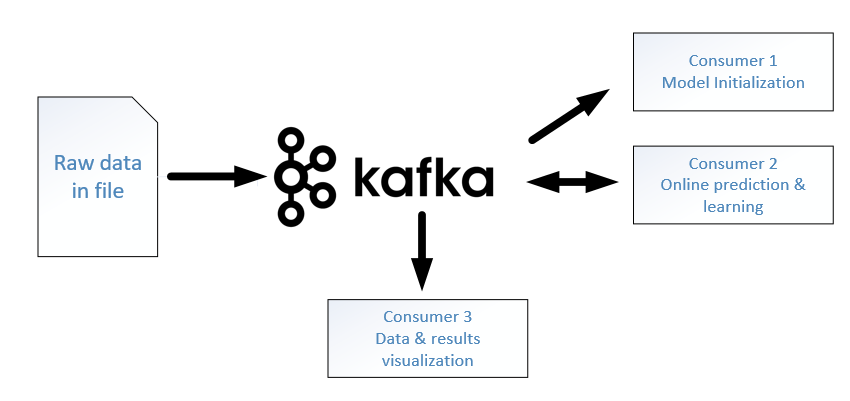
\includegraphics[width=10cm, height=5cm]{kafka}
\caption[Data stream pipeline]{Data stream pipeline}
\label{fig:kafka}
\end{figure}

\begin{algorithm}[t]
\SetKwInOut{Input}{input}
\Input{performanceThreshold, retrainDataSize}

\BlankLine 
needRetraining = False\;
retrainBuffer = [ ]\;
 \While{Batch data available}{
  batch, label = getBatchData()\;
  \eIf{len(retrainBuffer) == retrainDataSize}{retrain(retrainBuffer)\;}
	{
   	pred = predict(batch)\;
	result = evaluation(pred,label)\;
	\eIf{result >= performanceThreshold}{continue\;}{\eIf{label == "normal"}{retrainBuffer.append([B, label])\;}{continue\;}}
	}
 }
 \caption{Pipeline}
\label{alg:pipeline}
\end{algorithm}



\section{LSTMs-Autoencoder initialization}
\label{sec:initialization}

\subsection{Encoder-decoder architecture}
\label{sec:Encoder-decoder architecture}

The LSTMs-Autoencoder is consist of two LSTM units, one as encoder and the other one as decoder. The encoder inputs are fix length vectors with shape <MB, T, D>, where MB is the number of data windows contained in a mini-batch, T is the numbers of data points within each data window, and D represents the number of data dimensionality. Here, MB and T are learned as hyperparameter in the initialization phase. And on the decoder side, it will output exactly the same format data vector for each mini-batch. The LSTM unit copies its cell state for itself as one of the cell input at next timestamp. At the last timestamp of encoder, the cell state of LSTM unit is the hidden representation of the input data vector and copied to the decoder unit as initial cell state, so the hidden information can be passed to the decoder. The size of hidden layer representation vector, namely the size of cell state is another hyperparameter need to be learn in the initialization phase. The larger the hidden vector, the more information can be captured during the process, so it is a feature highly depends on the data. Similar to previous study \cite{seq2seq}, we also train the encoder and decoder with time series in reverse order. For example, if the input data fragment are data points from timestamp t1 to t2, then the decoder will predict data point at t2 at first, and then back to t1 step by step, while this trick makes the gradient escarpment between last state of encoder and first state of decoder smaller and easier to learn. 

In order to let the whole process happen online, the model initialization also utilizes streaming data. Once a small subset of streaming data is available, hyperparameters are learned, and then another dataset that consists only of normal data is collected from stream used for training.

\subsection{Anomaly detection mechanism}
\label{anomalydetection}
(Todo: reconstruction error, anomaly scoring, initialized scoring parameters used for online phase)



\section{Online learning}
\label{sec:Onlinelearning}
However, if we consider using the model for streaming data, the autoencoder might get outdated because of the relative small and simple initialization dataset and concept drift happed along with time. So the update of model is necessary. The main contribution of this paper is the incremental learning setting of the autoencoder model.

\subsection{Retraining trigger}
\label{trigger}

\subsection{Retraining dataset}
\label{data}


